\section{Solutions to exercises}
\label{sec:solutions}

\subsection{The optimal discriminator strategy}
\label{sec:opt_d_soln}

Our goal is to minimize
\begin{equation}
  J^{(D)}(\vtheta^{(D)}, \vtheta^{(G)}) = -\frac{1}{2} \E_{\vx \sim \pdata} \log D(\vx) - \frac{1}{2} \E_{\vz} \log \left(1 - D\left( G(z) \right) \right)
\end{equation}
in function space, specifying $D(\vx)$ directly.

We begin by assuming that both $\pdata$ and $\pmodel$ are nonzero everywhere.
If we do not make this assumption, then some points are never visited during training,
and have undefined behavior.

To minimize $J^{(D)}$ with respect to $D$, we can write down the functional derivatives with
respect to a single entry $D(\vx)$, and set them equal to zero:
\[
\frac{\delta} {\delta D(\vx)} J^{(D)} = 0.
\]
By solving this equation, we obtain
\[
D^*(\vx) = \frac{ \pdata(\vx) } {\pdata(\vx) + \pmodel(\vx) }.
\]

Estimating this ratio is the key approximation mechanism used by GANs.

The process is illustrated in \figref{fig:ratio}.

\begin{figure}
\centering
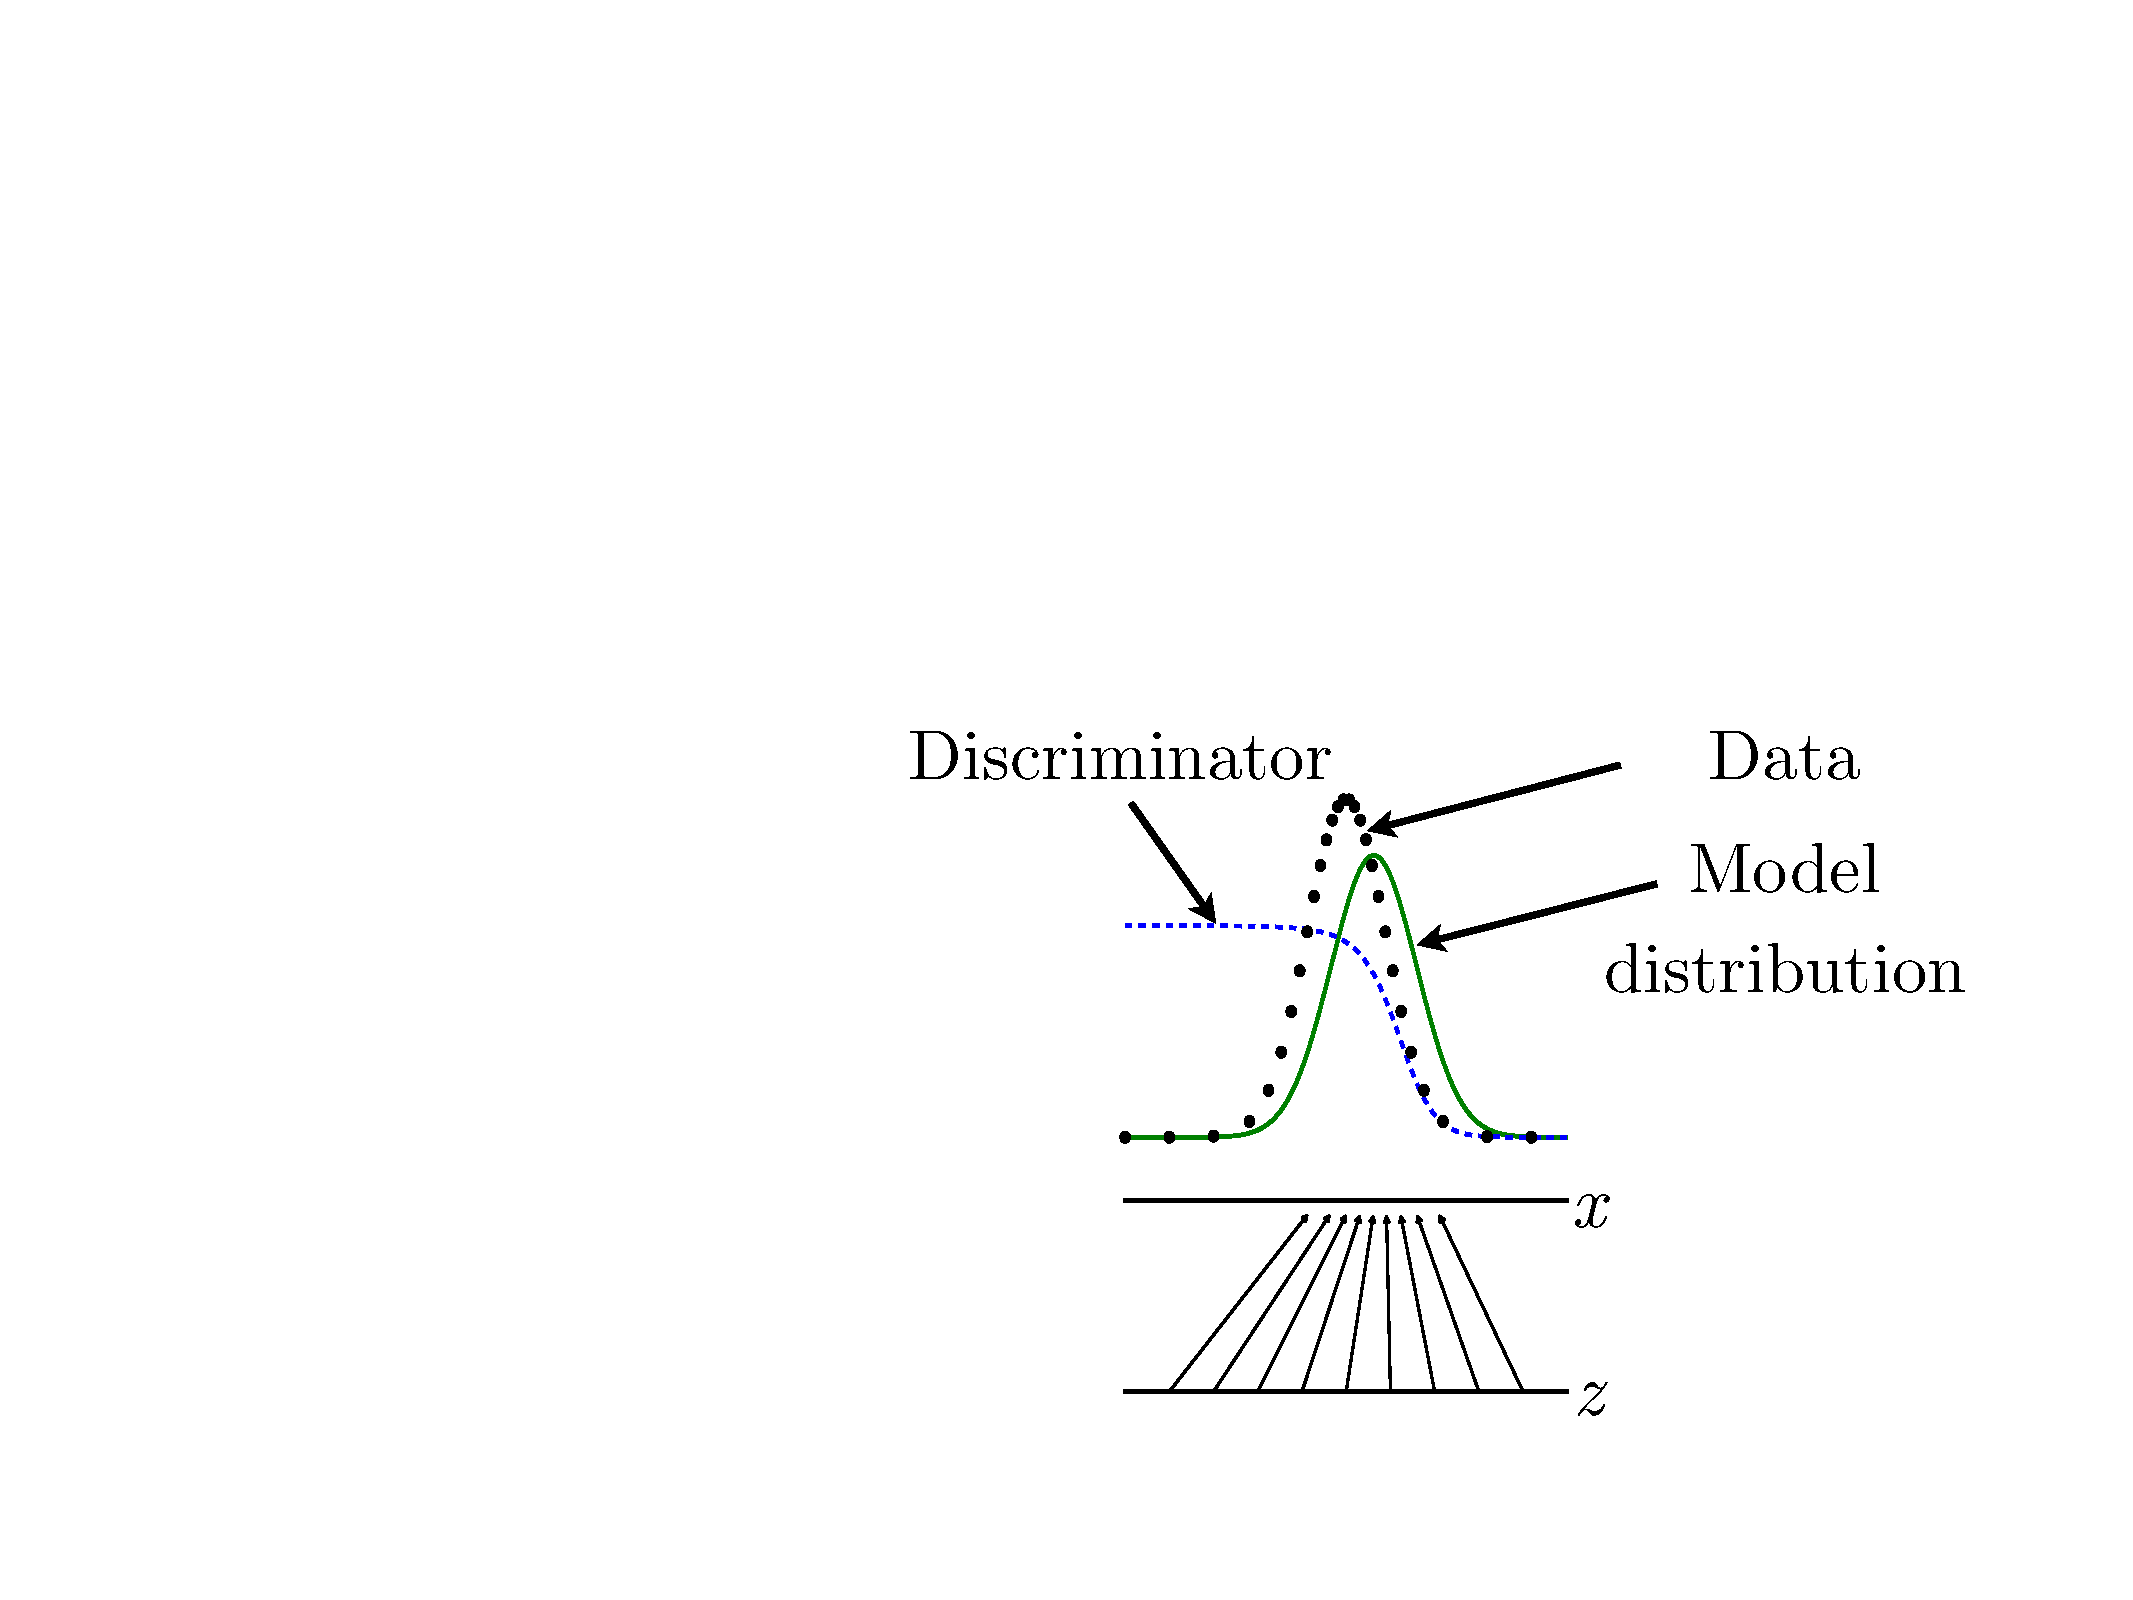
\includegraphics[width=\figwidth]{ratio}
\caption{
An illustration of how the discriminator estimates a ratio of
densities.
In this example, we assume that both $z$ and $x$ are one dimensional
for simplicity.
The mapping from $z$ to $x$ (shown by the black arrows) is non-uniform so that $\pmodel(x)$
(shown by the green curve) is
greater in places where $z$ values are brought together more densely.
The discriminator (dashed blue line) estimates the ratio between the data density (black dots)
and the sum of the data and model densities.
Wherever the output of the discriminator is large, the model density is too low, and wherever
the output of the discriminator is small, the model density is too high.
The generator can learn to produce a better model density by following the discriminator uphill;
each $G(z)$ value should move slightly in the direction that increases $D(G(z))$.
Figure reproduced from \citet{Goodfellow-et-al-NIPS2014-small}.
}
\label{fig:ratio}
\end{figure}


\subsection{Gradient descent for games}
\label{sec:xy_soln}

The value function
\[ V(x, y) = x y \]
is the simplest possible example of a continuous function with a saddle point.
It is easiest to understand this game by visualizing the value function in three
dimensions, as shown in \figref{fig:xy}.

\begin{figure}
\centering
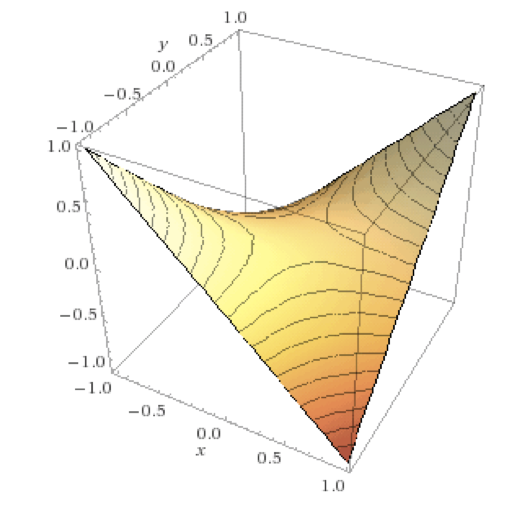
\includegraphics[width=\figwidth]{xy}
\caption{A three-dimensional visualization of the value function $V(x,y) = xy$.
  This is the canonical example of a function with a saddle point, at $x=y=0$.
}
\label{fig:xy}
\end{figure}

The three dimensional visualization shows us clearly that there is a saddle point
at $x=y=0$. This is an equilibrium of the game. We could also have found this point
by solving for where the derivatives are zero.

Not every saddle point is an equilibrium; we require that an infinitesimal perturbation
of one player's parameters cannot reduce that player's cost.
The saddle point for this game satisfies that requirement.
It is something of a pathological equilibrium because the value function is constant
as a function of each player's parameter when holding the other player's parameter
fixed.

To solve for the trajectory taken by gradient descent, we take the derivatives, and find that
\begin{align}
  \frac{\partial x}{\partial t} = - y(t) \\
  \frac{\partial y}{\partial t} = x(t). \label{eq:dy}
\end{align}
Diffentiating \eqref{eq:dy}, we obtain
\[
  \frac{\partial^2 y}{\partial t^2} = \frac{\partial x}{\partial t} = -y(t).
\]
Differential equations of this form have sinusoids as their set of basis functions
of solutions.
Solving for the coefficients that respect the boundary conditions, we obtain
\begin{align}
  x(t) = x(0) \cos(t) - y(0) \sin(t) \\
  y(t) = x(0) \sin(t) + y(0) \cos(t).
\end{align}

These dynamics form a circular orbit, as shown in \figref{fig:orbit}.
In other words, simultaneous gradient descent with an infinitesimal learning rate
will orbit the equilibrium forever, at the same radius that it was initialized.
With a larger learning rate, it is possible for simultaneous gradient descent to
spiral outward forever.
Simultaneous gradient descent will never approach the equilibrium.

\begin{figure}
  \center
  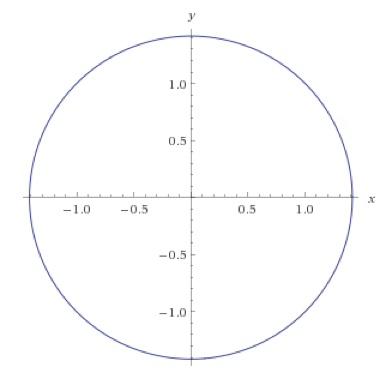
\includegraphics[width=\figwidth]{orbit}
  \caption{Simultaneous gradient descent with infinitesimal learning rate
    will orbit indefinitely at constant radius when applied to $V(x,y) = xy$,
    rather than approaching the equilibrium solution at $x=y=0$.
  }
  \label{fig:orbit}
\end{figure}

For some games, simultaneous gradient descent does converge, and for others,
such as the one in this exercise, it does not.
For GANs, there is no theoretical prediction as to whether simultaneous
gradient descent should converge or not.
Settling this theoretical question, and developing algorithms guaranteed to
converge, remain important open research problems.

\subsection{Maximum likelihood in the GAN framework}
\label{sec:mle_soln}

We wish to find a function $f$ such that the expected gradient of 
\begin{equation}
  J^{(G)} = \E_{\vx \sim p_g} f(\vx)
  \label{eq:cost_per_sample}
\end{equation}
is equal to the expected gradient of 
$\KL(\pdata \Vert p_g)$.

First we take the derivative of the KL divergence with respect to a parameter $\theta$:
\begin{equation}
  \frac{\partial}{\partial \theta} \KL(\pdata \Vert p_g) = - \E_{\vx \sim \pdata} \frac{\partial}{\partial \theta} \log p_g(\vx) .
\label{eq:mle_gradient}
\end{equation}

We now want to find the $f$ that will make the derivatives of \eqref{eq:cost_per_sample} match \eqref{eq:mle_gradient}.
We begin by taking the derivatives of \eqref{eq:cost_per_sample}:
\[
  \frac{\partial}{\partial \theta} J^{(G)} = \E_{\vx \sim p_g} f(x) \frac{\partial}{\partial \theta} \log p_g(\vx).
\]
To obtain this result, we made two assumptions:
\begin{enumerate}
  \item We assumed that $p_g(\vx) \geq 0$ everywhere so that we were able to use the identity $p_g(\vx) = \exp( \log p_g(\vx) ).$
  \item We assumed that we can use Leibniz's rule to exhange the order of differentiation and integration (specifically, that both the function and its derivative are continuous, and that the function vanishes for infinite values of $\vx$).
\end{enumerate}

We see that the derivatives of $J^{(G)}$ come very near to giving us what we want; the only problem is that
the expectation is computed by drawing samples from $p_g$ when we would like it to be computed by drawing
samples from $p_data$.
We can fix this problem using an importance sampling trick; by setting $f(x) = \frac{\pdata(\vx)}{p_g(\vx)}$
we can reweight the contribution to the gradient from each generator sample to compensate for it having
been drawn from the generator rather than the data.

Note that when constructing $J^{(G)}$ we must {\em copy} $p_g$ into $f(x)$ so that $f(x)$ has a derivative of
zero with respect to the parameters of $p_g$.
Fortunately, this happens naturally if we obtain the value of $\frac{\pdata(\vx)}{p_g(\vx)}$.

From \secref{sec:opt_d_soln}, we already know that the discriminator estimates the desired ratio.
Using some algebra, we can obtain a numerically stable implementation of $f(\vx)$.
If the discriminator is defined to apply a logistic sigmoid function at the output layer,
with $D(\vx) = \sigma( a(\vx) )$, then $f(x) = - \exp(a(\vx))$.

This exercise is taken from a result shown by \citet{Goodfellow-ICLR2015}.
From this exercise, we see that the discriminator estimates a ratio of densities
that can be used to calculate a variety of divergences.
